\documentclass[12pt]{article}

%environnement
\usepackage[letterpaper,margin=1in]{geometry}
\usepackage[utf8]{inputenc}
\usepackage{fontspec}
\usepackage[english]{babel}
\usepackage[parfill]{parskip}
\usepackage[style=ieee,backend=bibtex]{biblatex} %gestion bib
\usepackage{listings}
\usepackage{hyperref}
\usepackage[toc,acronym]{glossaries}
\usepackage[framemethod=TikZ]{mdframed} 
\usepackage{todonotes}
\usepackage[section]{placeins}
\hypersetup{
  pdftitle={},
  pdfborder={0 0 0}, %epaisseur box
  pdfauthor={Thomas LUINAUD},
}
\usepackage{tikz,tkz-tab}%package pour les tableaux de variations et de signes%
\usetikzlibrary{babel}
\usepackage{modules/tikzNetwork}
\usepackage{circuitikz}
\usetikzlibrary{positioning, automata, graphs, trees, fit, arrows.meta, shapes}
\usetikzlibrary{backgrounds,patterns,matrix,calc,shadows,plotmarks, circuits.logic.US}
\usetikzlibrary{decorations}
\usepackage{multirow}
\usepackage{modules/moeptikz}
%\usepackage{tabularx}
 %this file contains shape declaration and macro that define 
 %basic computer science shape for Hardware design.
 %this file should be include in the preamble
 
 \catcode`@=11

\pgfkeys{%
  /pgf/logicalbloc io north/.initial=5,
%  /pgf/logicalbloc io south/.initial=10,
%  /pgf/logicalbloc io east/.initial=10,
  /pgf/logicalbloc io west/.initial=10,
  /pgf/logicalbloc io north spacing/.initial=0.15cm,
%  /pgf/logicalbloc io south spacing/.initial=0.25cm,
%  /pgf/logicalbloc io east spacing/.initial=0.25cm,
  /pgf/logicalbloc io west spacing/.initial=0.20cm
}
\def\maxpins{100}


%stdChip
\pgfdeclareshape{logicalbloc}{
	\savedanchor\centerpoint{% 
		\pgf@x=.5\wd\pgfnodeparttextbox%
		\pgf@y=.5\ht\pgfnodeparttextbox%
		\advance\pgf@y by-.5\dp\pgfnodeparttextbox%
	  }
	  \anchor{center}{\centerpoint}
	  
	  \saveddimen\height{%
		\pgfmathsetlength\pgf@x{(\pgfkeysvalueof{/pgf/logicalbloc io west}+1)*\pgfkeysvalueof{/pgf/logicalbloc io west spacing}}%
	  }
	  \saveddimen\width{%
		\pgfmathsetlength\pgf@y{(\pgfkeysvalueof{/pgf/logicalbloc io north}+1)*\pgfkeysvalueof{/pgf/logicalbloc io north spacing}}%
	  }
	  \saveddimen{\yspacing}{\pgfmathsetlength\pgf@x{\pgfkeysvalueof{/pgf/logicalbloc io west spacing}}}	  
	  \saveddimen{\xspacing}{\pgfmathsetlength\pgf@y{\pgfkeysvalueof{/pgf/logicalbloc io north  spacing}}}
	  
	  \backgroundpath{%
		\pgfpathrectanglecorners{\pgfpointadd{\centerpoint}{\genbottomleftpoint}}%
		{\pgfpointadd{\centerpoint}{\gentoprightpoint}}%
	  }
 

	  \pgfmathloop%
	  \ifnum\pgfmathcounter>\maxpins\relax% 
	  \else%
		% Need to expand \pgfmathcounter
		\edef\marshal{\noexpand\anchor{io east \pgfmathcounter}}%
		\expandafter\marshal\expandafter{\expandafter\chippinanchorright\expandafter{\pgfmathcounter}}%
	  \repeatpgfmathloop%
	  
	  \pgfmathloop%
	  \ifnum\pgfmathcounter>\maxpins\relax% 
	  \else%
		% Need to expand \pgfmathcounter
		\edef\marshal{\noexpand\anchor{io north \pgfmathcounter}}%
		\expandafter\marshal\expandafter{\expandafter\chippinanchorupper\expandafter{\pgfmathcounter}}%
	  \repeatpgfmathloop%
	  
	  \pgfmathloop%
	  \ifnum\pgfmathcounter>\maxpins\relax% 
	  \else%
		% Need to expand \pgfmathcounter
		\edef\marshal{\noexpand\anchor{io south \pgfmathcounter}}%
		\expandafter\marshal\expandafter{\expandafter\chippinanchorbottom\expandafter{\pgfmathcounter}}%
	  \repeatpgfmathloop%
	  
	  \pgfmathloop%
	  \ifnum\pgfmathcounter>\maxpins\relax% 
	  \else%
		% Need to expand \pgfmathcounter
		\edef\marshal{\noexpand\anchor{io west \pgfmathcounter}}%
		\expandafter\marshal\expandafter{\expandafter\chippinanchorleft\expandafter{\pgfmathcounter}}%
	  \repeatpgfmathloop%
}

\def\genbottomleftpoint{%
%	\pgfmathsetlength{pgf@xb}{(\pgfkeysvalueof{/pgf/logicalbloc io north}+1)*\pgfkeysvalueof{/pgf/logicalbloc io north spacing}}%
%	\pgfmathsetlength{pgf@yb}{(\pgfkeysvalueof{/pgf/logicalbloc io west}+1)*\pgfkeysvalueof{/pgf/logicalbloc io west spacing}}%
%	\setlength{\pgf@xa}{1cm}
%	\setlength{\pgf@ya}{1cm}
%	\if \pgf@xb<\pgf@xa
%		\if \pgf@yb<\pgf@ya
%			\pgfpoint{-0.5cm}{-0.5cm}
%		\else
%			\pgfpoint{-0.5cm}{-(\pgfkeysvalueof{/pgf/logicalbloc io west}+1)*\pgfkeysvalueof{/pgf/logicalbloc io west spacing}/2}
%		\fi
%	\else
%		\if \pgf@yb<\pgf@ya
%			\pgfpoint{-(\pgfkeysvalueof{/pgf/logicalbloc io north}+1)*\pgfkeysvalueof{/pgf/logicalbloc io north spacing}/2}{-0.5cm}
%		\else
			\pgfpoint{-((\pgfkeysvalueof{/pgf/logicalbloc io north}+1)*\pgfkeysvalueof{/pgf/logicalbloc io north spacing})/2}{-((\pgfkeysvalueof{/pgf/logicalbloc io west}+1)*\pgfkeysvalueof{/pgf/logicalbloc io west spacing})/2}
%		\fi
%	\fi
}
\def\gentoprightpoint{%
%	\if {\pgfkeysvalueof{/pgf/logicalbloc io west} < \pgfkeysvalueof{/pgf/logicalbloc io east}}
%		\setlength{\pgf@xc}{1cm}
%	\else
%		\setlength{\pgf@xc}{1cm}
%	\fi
%	\if
%		\setlength{\pgf@xc}{1cm}
%	\else
%		\setlength{\pgf@xc}{1cm}
%	\fi
%	\pgfmathsetlength{pgf@xb}{(\pgfkeysvalueof{/pgf/logicalbloc io north}+1)*\pgfkeysvalueof{/pgf/logicalbloc io north spacing}}%
%	\pgfmathsetlength{pgf@yb}{(\pgfkeysvalueof{/pgf/logicalbloc io west}+1)*\pgfkeysvalueof{/pgf/logicalbloc io west spacing}}%
%	\setlength{\pgf@xa}{1cm}
%	\setlength{\pgf@ya}{1cm}
%	\if \pgf@xb<\pgf@xa
%		\if \pgf@yb<\pgf@ya
%			\pgfpoint{0.5cm}{0.5cm}
%		\else
%			\pgfpoint{0.5cm}{(\pgfkeysvalueof{/pgf/logicalbloc io west}+1)*\pgfkeysvalueof{/pgf/logicalbloc io west spacing}/2}
%		\fi
%	\else
%		\if \pgf@yb<\pgf@ya
%			\pgfpoint{(\pgfkeysvalueof{/pgf/logicalbloc io north}+1)*\pgfkeysvalueof{/pgf/logicalbloc io north spacing}/2}{0.5cm}
%		\else
			\pgfpoint{((\pgfkeysvalueof{/pgf/logicalbloc io north}+1)*\pgfkeysvalueof{/pgf/logicalbloc io north spacing})/2}{((\pgfkeysvalueof{/pgf/logicalbloc io west}+1)*\pgfkeysvalueof{/pgf/logicalbloc io west spacing})/2}
%		\fi
%	\fi
}


\def\genpointbottom#1{
\pgfpoint{(\pgfkeysvalueof{/pgf/logicalbloc io north}+1)*\pgfkeysvalueof{/pgf/logicalbloc io north spacing}/2-#1*\xspacing}{-(\pgfkeysvalueof{/pgf/logicalbloc io west}+1)*\pgfkeysvalueof{/pgf/logicalbloc io west spacing}/2}
}

\def\chippinanchorbottom#1{%
	  % When this macro is called,
	  % \centerpoint, \height and \chipspacing will be defined.
	  %\pgfpointadd{\centerpoint}{\pgfpoint{\width/2-#1*\xspacing}{-\height/2}}%
	  \pgfpointadd{\centerpoint}{\genpointbottom{#1}}%
}

\def\genpointupper#1{
\pgfpoint{(\pgfkeysvalueof{/pgf/logicalbloc io north}+1)*\pgfkeysvalueof{/pgf/logicalbloc io north spacing}/2-#1*\xspacing}{(\pgfkeysvalueof{/pgf/logicalbloc io west}+1)*\pgfkeysvalueof{/pgf/logicalbloc io west spacing}/2}
}

\def\chippinanchorupper#1{%
	  % When this macro is called,
	  % \centerpoint, \height and \chipspacing will be defined.
	  \pgfpointadd{\centerpoint}{\genpointupper{#1}}%
}

\def\genpointleft#1{
\pgfpoint{-(\pgfkeysvalueof{/pgf/logicalbloc io north}+1)*\pgfkeysvalueof{/pgf/logicalbloc io north spacing}/2}{(\pgfkeysvalueof{/pgf/logicalbloc io west}+1)*\pgfkeysvalueof{/pgf/logicalbloc io west spacing}/2-#1*\yspacing}
}

\def\chippinanchorleft#1{%
	  % When this macro is called,
	  % \centerpoint, \height and \chipspacing will be defined.
	  \pgfpointadd{\centerpoint}{\genpointleft{#1}}%
}

\def\genpointright#1{
\pgfpoint{(\pgfkeysvalueof{/pgf/logicalbloc io north}+1)*\pgfkeysvalueof{/pgf/logicalbloc io north spacing}/2}{(\pgfkeysvalueof{/pgf/logicalbloc io west}+1)*\pgfkeysvalueof{/pgf/logicalbloc io west spacing}/2-#1*\yspacing}
}
\def\chippinanchorright#1{%
	  % When this macro is called,
	  % \centerpoint, \height and \chipspacing will be defined.
	  \pgfpointadd{\centerpoint}{\genpointright{#1}}%
}

\catcode`@=12
\usepackage{cancel}%package pour barrer et simplifier%
\usepackage{amsmath}%matrice%
\usepackage{stmaryrd}
\usepackage{textcomp}
\usepackage{pstricks}
\usepackage{pdftricks, pstricks-add}
\usepackage{pgfplots}
\usepackage{caption}
\usepackage{subfig}
\usepackage{pdfpages}
	
\hyphenation{contien-nent}

\usepackage[nounderscore]{syntax}
\newlength\grammarLongest
\newlength\grammarLeftMargin
\makeatletter
\newenvironment{grammarC}[1]{%
\list{}{%
\settowidth\grammarLongest{#1}
\setlength\grammarLeftMargin{\dimexpr0.5\linewidth-0.5\grammarLongest}
\labelwidth\grammarindent%
\leftmargin\dimexpr\grammarindent+\grammarLeftMargin\relax%
\advance\grammarindent\labelsep
\itemindent\z@%
\listparindent\z@%
\parsep\grammarparsep%
}%
\let\\\@normalcr
\syntaxShortcuts\relax\relax%
\def\alt{\\\llap{\textbar\quad}}%
\def\gr@setpar{%
\def\par{%
\parshape\@ne\@totalleftmargin\linewidth%
\@@par%
\catcode`\<12%
\everypar{%
\everypar{}%
\catcode`\<\active%
\gr@implitem%
}%
}%
}%
\gr@setpar%
\par%
\let\gr@leftsq\[%
\let\gr@rightsq\]%
\def\gr@endsyntdiag]{\end{syntdiag}\gr@setpar\par}%
\def\[{\@ifnextchar[{\begin{syntdiag}\@gobble}\gr@leftsq}%
\def\]{\@ifnextchar]\gr@endsyntdiag\gr@rightsq}%
}{%
\@newlistfalse%
\everypar{}%
\endlist%
}
\makeatother
\usepackage{varwidth}

\usepackage{tabularx}
\usepackage{csvsimple}
\usepackage{float}
\usepackage{amssymb}
\usepackage[linesnumbered,lined, french, frenchkw, figure, noend]{algorithm2e}

\newcommand{\inputFig}[2]{\IfFileExists{#1}{\input{#1}}{\missingfigure[figheight=3cm]{#2}}}

\newsavebox{\tempbox}
\newsavebox{\tempboxi}


% Title Page
\title{Étape 2 du projet de compilateur \\ Rapport}
\author{Thomas Luinaud \\ Francis de Ladurantaye}


\begin{document}
\begin{titlepage}
  \maketitle
\end{titlepage}

\section{Structure logicielle}
\begin{figure}[h]
	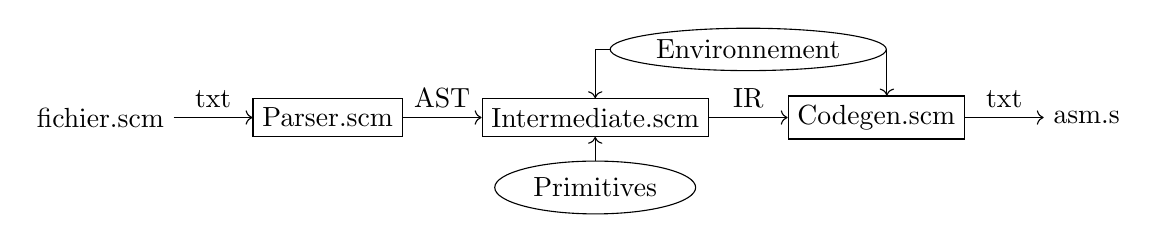
\begin{tikzpicture}
		\node[](file) {fichier.scm};
		\node[draw, right=of file] (parser) {Parser.scm};
		\node[draw, right=of parser] (intermediate) {Intermediate.scm};
		\node[draw, right=of intermediate] (codegen) {Codegen.scm};
		\node[right=of codegen] (asm) {asm.s};
		\node[below =0.3cm of intermediate, ellipse, draw](prims) {Primitives};
		
		\path[draw, ->] (prims) -- (intermediate);
		\path[->] (file) edge node [above] {txt} (parser)
				  (parser) edge node [above] {AST} (intermediate)
				  (intermediate) edge node (outIR)  [above] {IR} (codegen)
				  (codegen) edge node [above] {txt} (asm);
		\node[above =0.1cm of outIR, ellipse, draw, inner sep=2pt](symbTable) {Environnement};
		\path[draw, ->] (symbTable) -| (intermediate);
		\path[draw, ->] (symbTable) -| (codegen.north -| symbTable.east);
	\end{tikzpicture}
	\caption{structure du compilateur}
\end{figure}

\section{Code intermédiaire}
Cette section présente les choix pour le code intermédiaire.

\begin{table}[h]
	\begin{tabular}{|c|l|}
		\hline
		code intermediaire & description \\ \hline
		\texttt{print\_char} & affiche un élément \\ \hline
		\texttt{print\_num} & affiche un élément \\ \hline
		
		\texttt{push\_lit} \emph{val}& ajoute un litteral sur la pile\\ \hline
		\texttt{push\_glo} \emph{name} & ajouter la valeur d'une variable\\ \hline
		\texttt{push\_loc} \emph{i} & empiler la valeur d'une variable locale. \emph{i} est l'index sur la pile\\ \hline
		\texttt{add}	& depiler deux valeurs et les ajouter \\ \hline
		\texttt{sub}	& depiler deux valeurs et les soustraire \\ \hline
		\texttt{mul}	& depiler deux valeurs et les multiplier \\ \hline
		\texttt{div}	& depiler deux valeurs et les diviser \\ \hline
		\texttt{call} \emph{nargs} & appeler une fonction avec \emph{nargs} argument\\ \hline
		\texttt{ret} \emph{i} & retourne la valeur à l'index \emph{i} de la pile\\  \hline
		\texttt{cmp} & dépile deux valeurs et les compare \\ \hline
		\texttt{modulo} & dépile deux valeurs et fait le modulo \\ \hline
        \texttt{remainder} & dépile deux valeurs et fait le remainder \\ \hline
        \texttt{quotient} & dépile deux valeurs et fait le quotient \\ \hline
        \texttt{lesser} & résultat de la comparaison est plus petit \\ \hline
        \texttt{equal} & résultat de la comparaison est égal \\ \hline
        \texttt{jmp} \emph{étiquette} & va à la position spécifiée\\ \hline 
	\end{tabular}
\end{table}

\newpage

\section{Spécification du problème}

À cette étape du projet, il nous fallait être en mesure de compiler, en plus des entiers et des booléens déjà supportés à l'étape 1, les listes, les caractères, les chaînes de caractères ainsi que les constantes littérales structurées. Par ailleurs, nous devions supporter la définition et la mutation de variables globales et permettre la déclaration et les appels de fonction (lambda-expressions inclues). Une fois en mesure de compiler ce qui précède, ces outils devaient être utilisés pour construire la liste d'opérations primitives du langage ainsi qu'une biliothèque de fonctions prédéfinies, servant principalement à intéragir avec les nouveaux types de données supportés. Enfin, nous devions ajouter une phase d'expansion de macros pour les macros \texttt{cond}, \texttt{and}, \texttt{or}, \texttt{begin}, \texttt{let*}, \texttt{letrec} et \texttt{let} nommé afin de permettre à notre compilateur de supporter des énoncés conditionnels plus complexes et la définition de variables locales.

\subsection{Opérations primitives}

À la fin de cette étape, en plus de ce qui était demandé à l'étape 1, il nous était donc demandé d'implanter les opérations primitives suivantes :

\begin{itemize}
\item (\texttt{\$number?} \textit{expr}) : test de type pour les entiers
\item (\texttt{\$read-char}) : lecture d'un caractère sur stdin
\item (\texttt{\$write-char} \textit{expr}) : écriture d'un caractère sur stdout
\item (\texttt{\$integer->char} \textit{expr}) : conversion d'entier vers caractère
\item (\texttt{\$char->integer} \textit{expr}) : conversion de caractère vers entier
\item (\texttt{\$char?} \textit{expr}) : test de type pour les caractères
\item (\texttt{\$make-string} \textit{expr}) : création d'une chaîne de caractères ayant la longueur indiquée 
\item (\texttt{\$string-ref} \textit{$expr_1$ $expr_2$}) : extraction d'un caractère à un certain index
\item (\texttt{\$string-set!} \textit{$expr_1$ $expr_2$ $expr_3$}) : modification d'un caractère à un certain index
\item (\texttt{\$string-length} \textit{expr}) : nombre de caractères dans la chaîne de caractères
\item (\texttt{\$string?} \textit{expr}) : test de type pour les chaînes de caractères
\item (\texttt{\$cons} \textit{$expr_1$ $expr_2$}) : création d'une paire
\item (\texttt{\$car} \textit{expr}) : extraction du champ car
\item (\texttt{\$cdr} \textit{expr}) : extraction du champ cdr
\item (\texttt{\$set-car!} \textit{$expr_1$ $expr_2$}) : modification du champ car
\item (\texttt{\$set-cdr!} \textit{$expr_1$ $expr_2$}) : modification du champ cdr
\item (\texttt{\$pair?} \textit{expr}) : test de type pour les paires
\item (\texttt{\$procedure?} \textit{expr}) : test de type pour les fonctions
\item (\texttt{\$eq?} \textit{$expr_1$ $expr_2$}) : test d'identité
\end{itemize}

\subsection{Fonctions prédéfinies}

Une fois ajouté le support des opérations précédentes, nous avions à les utiliser pour la construction de cette bibliothèque de fonctions prédéfinies :

\begin{itemize}
\item (\texttt{not} \textit{expr}) : inverse booléen
\item (\texttt{boolean?} \textit{expr}) : test de type pour les booléens
\item (\texttt{null?} \textit{expr}) : test de type pour la liste vide
\item (\texttt{member} \textit{$expr_1$ $expr_2$}) : test d'appartenance
\item (\texttt{assoc} \textit{$expr_1$ $expr_2$}) : recherche dans une liste d'association
\item (\texttt{append} \textit{$expr_1$ $expr_2$}) : concaténation de listes
\item (\texttt{reverse} \textit{expr}) : renverser une liste
\item (\texttt{length} \textit{expr}) : longueur d'une liste
\item (\texttt{map} \textit{$expr_1$ $expr_2$}) : map sur les listes
\item (\texttt{char=?} \textit{$expr_1$ $expr_2$}) : test d'égalité de caractères
\item (\texttt{char<?} \textit{$expr_1$ $expr_2$}) : test < sur les caractères
\item (\texttt{string=?} \textit{$expr_1$ $expr_2$}) : test d'égalité sur les chaîens de caractères
\item (\texttt{string<?} \textit{$expr_1$ $expr_2$}) : test < sur les chaînes de caractères
\item (\texttt{eqv?} \textit{$expr_1$ $expr_2$}) : test d'équivalence
\item (\texttt{equal?} \textit{$expr_1$ $expr_2$}) : test d'égalité structurelle
\item (\texttt{read}) : lecture d'une donnée Scheme sur stdin
\item (\texttt{write} \textit{expr}) : écriture dune donnée Scheme sur stdout
\end{itemize}

Malheureusement, comme il sera expliqué plus en détail dans les sections subséquentes, nous n'avons réussi à implémenter qu'un mince ensemble de ces opérations et fonctions.

\section{Méthodologie}

Comme nous savions dès le départ que l'implantation des opérations primitives et des fonctions prédéfinies requerrait le support des définitions et appels de fonctions, c'est donc à cela que nous nous sommes d'abord attaqués. Ce faisant, nous avons consacré la majeure partie de notre énergie à cette tâche afin d'éviter de devoir réécrire du code à plusieurs reprises. Comme le support des définitions et appels de fonctions demandait de savoir gérer la conversion de fermeture adéquatement, c'est par cela que nous avons commencé.

Autrement, dans nos moments de désespoir, nous avons travaillé sur les modules ne nécessitant pas de savoir gérer les fermetures. Parmi ces modules, on compte la génération de la représentation intermédiaire, la traduction de la représentation intermédiaire en code assembleur et la phase d'expansion de macros, tâches avec lesquelles nous avons eu plus de succès.

\section{Problèmes rencontrés}

\subsection{Conversion de fermetures}

La conversion des fermetures a de loin été ce qui nous a causé le plus de problèmes. Il nous fallut un temps considérable pour commencer à cerner ce qui se passait au sein du fichier \texttt{closure-conv.scm} et bien que nous croyons plutôt bien comprendre les différentes étapes de la conversion de fermeture et leurs justifications, ce serait un euphémiste d'affirmer que nous ne serions point en mesure de le réécrire si nous avions à le faire. De plus, nous ne comprenions initialement pas comment traiter les \text{make-closure} afin d'en produire la représentation intermédiaire. Heureusement nous avons commencé à voir la lumière au bout du tunnel dans les deux derniers jours mais cela ne nous a pas laissé le temps d'implanter les opérations et fonctions demandées.

\subsection{Représentation intermédiaire}

La grande difficulté que nous avons eue au niveau de la représentation intermédiaire fut celle mentionnée au paragraphe précédent. Nous nous sommes posé un grand nombre de questions sur la façon de produire cette représentation intermédiaire lorsque nous tombions sur des expressoins de la forme \texttt{(define fun (lambda (x) ... ))}. Sachant qu'une telle expression ne doit pas exécuter le code de la lambda-expression, nous avions réalisé que ce n'était pas à cet endroit que nous devions produire le code de la représentation intermédiaire de cette lambda-expression. Comme il n'était pas possible de simplement ignorer le corps de la lambda-expression lors de la production de la représentation intermédiaire pour y revenir plus tard, nous avons fini par supposer qu'il fallait la produire lors de notre passage mais en la gardant en mémoire dans une sorte d'environnement pour les lambda-expressions. Ainsi, il serait possible d'y avoir accès plus tard lors de la génération de code assembleur, ce qui permettrait de les écrire à l'extérieur de la fonction \texttt{main}.

\subsection{Expansion de macros}

L'implantation de la phase d'expansion de macros nous a posé certains problèmes, mais bien moindres que pour la conversion des fermetures et la production de la représentation intermédiaire. Une des difficultés rencontrée a été de comprendre où devait avoir lieu l'expansion. Cela était dû au fait que nous avions déjà implanté la majorité des macros demandées lors de l'étape 1, mais que nous l'avions fait en utilisant \texttt{define-macro}. Nous nous demandions donc comment effectuer les substitutions une fois la phase de \textit{parsing} terminée, et ce de façon récursive afin d'éliminer aussi les macros qui seraient apparues suite à une première substitution. Afin de pallier au problème, nous avons opté pour la réécriture des macros, cette fois-ci en faisant usage des capacités de \textit{pattern matching} offertes par la macro \texttt{match} vue en classe. Il devenait donc très simple, en effectuant une substitution, d'appeler récursivement la fonction d'expansion de macros sur le code de remplacement.

Aussi en lien avec l'expansion des macros, il nous fut particulièrement difficile de trouver comment substituer correctement la forme \textit{letrec}. La liaison des variables aux expressions se faisant en trois temps (création des variables, calcul de expressions et enfin liaison des résultats aux variables), cette macro dépasse largement les formes \texttt{let} et \texttt{let*} en ce qui a trait au niveau de complexité de son implémentation. Nous y sommes toutefois arrivés et en sommes très fier.

\section{Résultats des tests unitaires}

Comme la gestion des fermetures et l'ajout de la représentation intermédiaire ont demandé une refonte majeure de notre compilateur, le temps nous a malheureusement (grandement) manqué pour implanter ce qui était démandé. Notre compilateur se trouve présentement dans un état dans lequel la majorité des tests unitaires n'arrivent pas à compiler correctement et il est donc difficile de présenter les résultats à ces tests. Toutefois, nous pouvons affirmer que les tests simples (addition, soustraction, multiplication, quotient, modulo) fonctionnent s'ils ne contiennent qu'un seul niveau d'imbrication de \texttt{let}. En temps normal, nous devrions parvenir à passer avec succès l'ensemble des tests d'ici environ une semaine.

\section{Atteinte des objectifs}

Tel qu'expliqué lors des sections précédentes, la refonte majeure du compilateur nous a littéralement complètement empêché d'arriver à atteindre les objectifs associés à l'étape 2. Cependant, nous prenons cela avec philosophie comme nous savons que cette refonte était nécessaire et qu'elle ne sera pas à refaire. Nous aurions cependant préféré savoir dès la première étape qu'avoir une représentation intermédiaire est une quasi nécessité. Cela nous aurait permis de penser différemment notre compilateur dès le départ, nous évitant peut-être cette refonte complète qui a plombé notre atteinte des objectifs.

\newpage

\section{Annexes}

\subsection{Grammaire}
Voici notre grammaire (approximative et fortement inspiré de la documentation R7RS) pour l'implantation de notre parseur :
\begin{figure}[h!]
  %commande \alt permet de mettre une | en début de ligne pour continuer une expression en mettant un retour à la ligne
%grammarC permet de centrer le code le paramètre contient la plus longue ligne

\begin{grammarC}{<expression> ::= <expression-ent> | <opérateur> <entiers>}
  
  <datum> ::= <datum simple> | <procédure> | <abréviation>
  
  <abréviation> ::= <abrev> <datum>
  
  <abrev> ::= "'" | \space "\`" | ","
  
  <procédure> ::= ( <opérateur> <données> )
  
  <datum simple> ::= <booléen> | <nombre> | <symbole> | <string>
  
  <booléen> ::= \#t | \#f
  
  <string> ::= \verb|"| <element string>* \verb|"|
  
  <element string> ::= <tout caractère différent de \verb|" \|  > | \verb|\"| | \verb|\\|
  
  <opérateur> ::= "+" | "-" | "*" | "=" | "<" | <symbol>
  
  <nombre> ::= <valeurNeg> | <valeurPos>
  
  <valeurNeg> ::= "-" <entier>
  
  <valeurPos> ::= <signePos> <entier>
  
  <entier> ::= <digit> <entier> | <digit>
  
  <signePos> ::= "+" | $\epsilon$ 
  
  <digit> ::= '0' | '1' | '2' | '3' | '4' | '5' | '6' | '7' | '8' | '9'		
  
\end{grammarC}

  \caption{Représentation EBNF de la grammaire à supporter.}
\end{figure}

\end{document}          
